\chapter{Experimental Results}

\section{Quantitative Comparison}

Table \ref{tab:main_results} reports the main quantitative results on the held-out L506 patient. The low-dose input has 29.2489 dB PSNR, 0.8759 SSIM, and 14.2416 RMSE. All learned models substantially improve the low-dose input, confirming that supervised denoising is effective under the current paired setting. The CTformer result is reported with the updated 100000-iteration continuation checkpoint.

\begin{table}[!htbp]
    \centering
    \caption{Quantitative results on the held-out L506 test patient.}
    \renewcommand{\arraystretch}{1.25}
    \small
    \begin{tabular}{lcccc}
        \hline
        Method & Checkpoint & PSNR \(\uparrow\) & SSIM \(\uparrow\) & RMSE \(\downarrow\) \\
        \hline
        Low-dose input & -- & 29.2489 & 0.8759 & 14.2416 \\
        \hline
        CTformer & 54718 & 32.3852 & 0.9026 & 9.8366 \\
        \hline
        CTformer & 100000 & 32.6688 & 0.9067 & 9.5197 \\
        \hline
        RED-CNN & 9500 & 32.6656 & 0.9067 & 9.4867 \\
        \hline
        CTRestormer & 11500 & 32.1294 & 0.8997 & 10.0689 \\
        \hline
        CTRestormer & 16500 & 32.3584 & 0.9049 & 9.8145 \\
        \hline
        CTRestormer & 21500 & \textbf{32.6738} & \textbf{0.9096} & \textbf{9.4842} \\
        \hline
    \end{tabular}
    \label{tab:main_results}
\end{table}

The updated CTformer 100000 checkpoint reaches 32.6688 dB PSNR, 0.9067 SSIM, and 9.5197 RMSE. Compared with RED-CNN 9500, it is slightly higher in PSNR by 0.0032 dB and has the same four-decimal SSIM, while RED-CNN remains slightly better in RMSE by 0.0330. The best CTRestormer checkpoint still gives the best overall metrics in this table, reaching 32.6738 dB PSNR, 0.9096 SSIM, and 9.4842 RMSE. Compared with CTformer at the same 21500-iteration checkpoint, CTRestormer improves PSNR by 0.8279 dB, improves SSIM by 0.0085, and reduces RMSE by 1.0418.

\begin{figure}[!htbp]
    \centering
    
\includegraphics[width=0.85\textwidth]{images/metrics_comparison.png}
    \caption{Metric comparison of selected final results on the held-out L506 patient. CTformer uses the updated 100000-iteration checkpoint.}
    \label{fig:metrics}
\end{figure}


\section{Estimated Training-Budget Comparison}

Iteration count is not a fair proxy for computational budget because the three models have different architectures, different per-iteration costs, and different training code. The raw elapsed fields in the historical logs also cannot be directly accumulated because several runs were interrupted and later resumed. To still provide a useful training-budget reference, this thesis estimates a 100-minute training budget from continuous checkpoint-saving segments that show no obvious long interruption. This estimate is not a strict same-wall-clock experiment, but it is more informative than comparing only final selected checkpoints.

Table \ref{tab:estimated_time_budget} shows the speed-estimation protocol. For each model, a representative continuous checkpoint segment is used to estimate iterations per minute. The estimated 100-minute iteration count is then rounded to the nearest available or evaluated checkpoint. For CTformer, the 70000 checkpoint should be read as a 100-minute-equivalent checkpoint estimated from the observed checkpoint-saving speed, not as proof that the whole training history up to 70000 iterations took only 100 minutes.

\begin{table}[!htbp]
    \centering
    \caption{Estimated 100-minute training budget from representative continuous checkpoint segments.}
    \renewcommand{\arraystretch}{1.25}
    \small
    \begin{tabular}{lccccc}
        \hline
        Model  & Segment time & Iter/min & Estimated 100-min iter & Used checkpoint \\
        \hline
        CTformer  & 49.6 min & 705.1 & 70505 & 70000 \\
        \hline
        RED-CNN  & 95.9 min & 93.8 & 9380 & 9500 \\
        \hline
        CTRestormer & 80.0 min & 137.5 & 13754 & 14000 \\
        \hline
    \end{tabular}
    \label{tab:estimated_time_budget}
\end{table}

Table \ref{tab:estimated_time_results} reports the corresponding test metrics. Under this estimated 100-minute budget, RED-CNN gives the best PSNR and RMSE. CTRestormer is slightly higher than CTformer in SSIM, but its PSNR and RMSE are not better at this estimated early budget. This result is useful because it prevents overstating the proposed model: CTRestormer is not the most efficient short-budget model in the current implementation. Its advantage appears more clearly after longer training, as shown by the final 21500-iteration checkpoint in Table \ref{tab:main_results}.

\begin{table}[!htbp]
    \centering
    \caption{Estimated 100-minute training-budget comparison on L506.}
    \renewcommand{\arraystretch}{1.25}
    \small
    \begin{tabular}{lccccc}
        \hline
        Model & Used checkpoint & Approx. epoch & PSNR \(\uparrow\) & SSIM \(\uparrow\) & RMSE \(\downarrow\) \\
        \hline
        CTformer & 70000 & 129.2 & 32.4017 & 0.9012 & 9.8020 \\
        \hline
        RED-CNN & 9500 & 69.9 & \textbf{32.6656} & \textbf{0.9067} & \textbf{9.4867} \\
        \hline
        CTRestormer & 14000 & 12.9 & 32.3718 & 0.9044 & 9.8020 \\
        \hline
    \end{tabular}
    \label{tab:estimated_time_results}
\end{table}

Table \ref{tab:same_iter} reports a same-iteration comparison between CTformer and CTRestormer at 21500 iterations because both checkpoints exist in the current experiment records. This table is useful for showing relative progress at the same checkpoint index, but it should not be interpreted as a same-compute comparison. RED-CNN is not included in this table because its saved checkpoint schedule and training code are different.

\begin{table}[!htbp]
    \centering
    \caption{Same-iteration comparison between CTformer and CTRestormer on L506.}
    \renewcommand{\arraystretch}{1.25}
    \small
    \begin{tabular}{lcccc}
        \hline
        Model & Iteration & PSNR \(\uparrow\) & SSIM \(\uparrow\) & RMSE \(\downarrow\) \\
        \hline
        CTformer & 21500 & 31.8459 & 0.9011 & 10.5260 \\
        \hline
        CTRestormer & 21500 & \textbf{32.6738} & \textbf{0.9096} & \textbf{9.4842} \\
        \hline
    \end{tabular}
    \label{tab:same_iter}
\end{table}

This comparison shows that CTRestormer is much stronger than CTformer at the same iteration count. The reason is not only parameter count: CTRestormer has a restoration-oriented multi-scale encoder-decoder, skip fusion, local convolutional mixing inside attention and feed-forward branches, and residual output prediction. CTformer becomes competitive only after much longer continuation training to 100000 iterations, while CTRestormer reaches comparable or better metrics at 21500 iterations. RED-CNN remains a strong baseline, but its training loop and saved checkpoint schedule are different, so it is more appropriately discussed in the selected-checkpoint comparison in Table \ref{tab:main_results} and the estimated time-budget comparison in Table \ref{tab:estimated_time_results}.

\section{Qualitative Comparison}

Figure \ref{fig:qualitative} shows a representative qualitative result for slice L506\_88. Qualitative comparison is necessary because PSNR and SSIM do not directly reveal texture quality, boundary sharpness, or possible over-smoothing. The CTformer panel uses the updated 100000-iteration checkpoint. The low-dose input contains stronger noise texture, while the denoised outputs are visually closer to the normal-dose target. The comparison should be interpreted together with residual maps in Chapter 6.

\begin{figure}[!htbp]
    \centering
    
\includegraphics[width=0.95\textwidth]{images/qualitative_l506_88_ctformer.png}
    \caption{Representative qualitative comparison for slice L506\_88. All panels are shown under the same display setting.}
    \label{fig:qualitative}
\end{figure}

Two additional slices are included to make the visual comparison less dependent on a single representative image. Slice L506\_45 was selected from an earlier axial range with relatively high input-target error within that range, while slice L506\_180 has the highest input-target RMSE among the scanned L506 slices. These two cases cover different anatomical regions and make denoising differences easier to inspect.

\begin{figure}[!htbp]
    \centering
    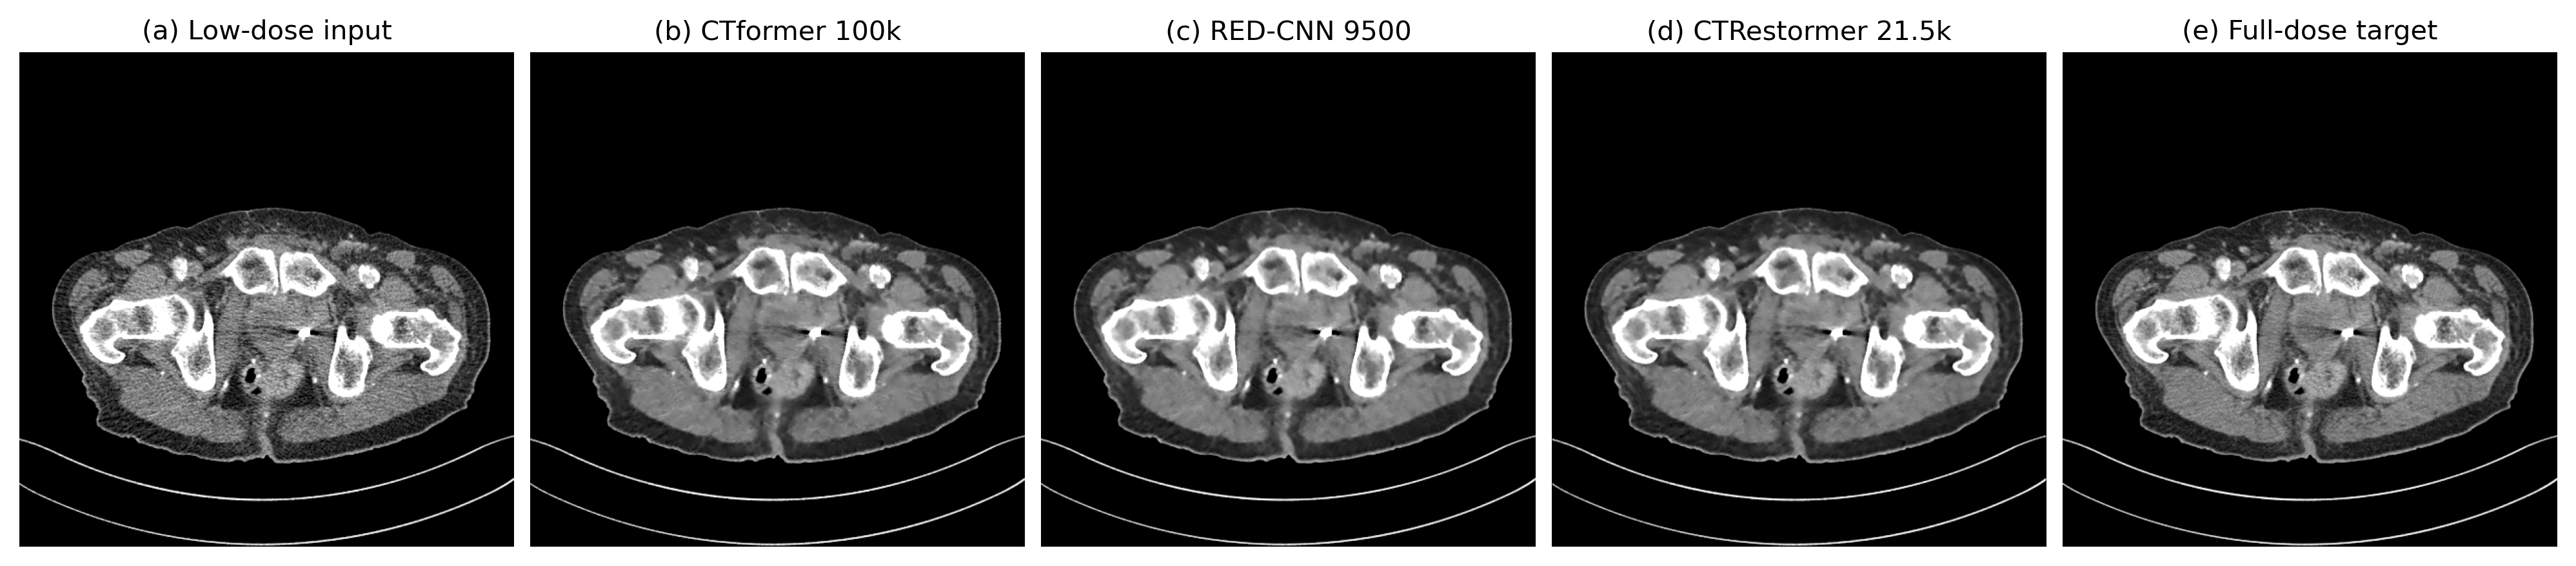
\includegraphics[width=0.95\textwidth]{images/qualitative_l506_45_comparison.png}
    \caption{Additional qualitative comparison for slice L506\_45. This slice shows a pelvic region and provides a separate visual case from the abdominal slice used in Figure \ref{fig:qualitative}.}
    \label{fig:qualitative_l506_45}
\end{figure}

\begin{figure}[!htbp]
    \centering
    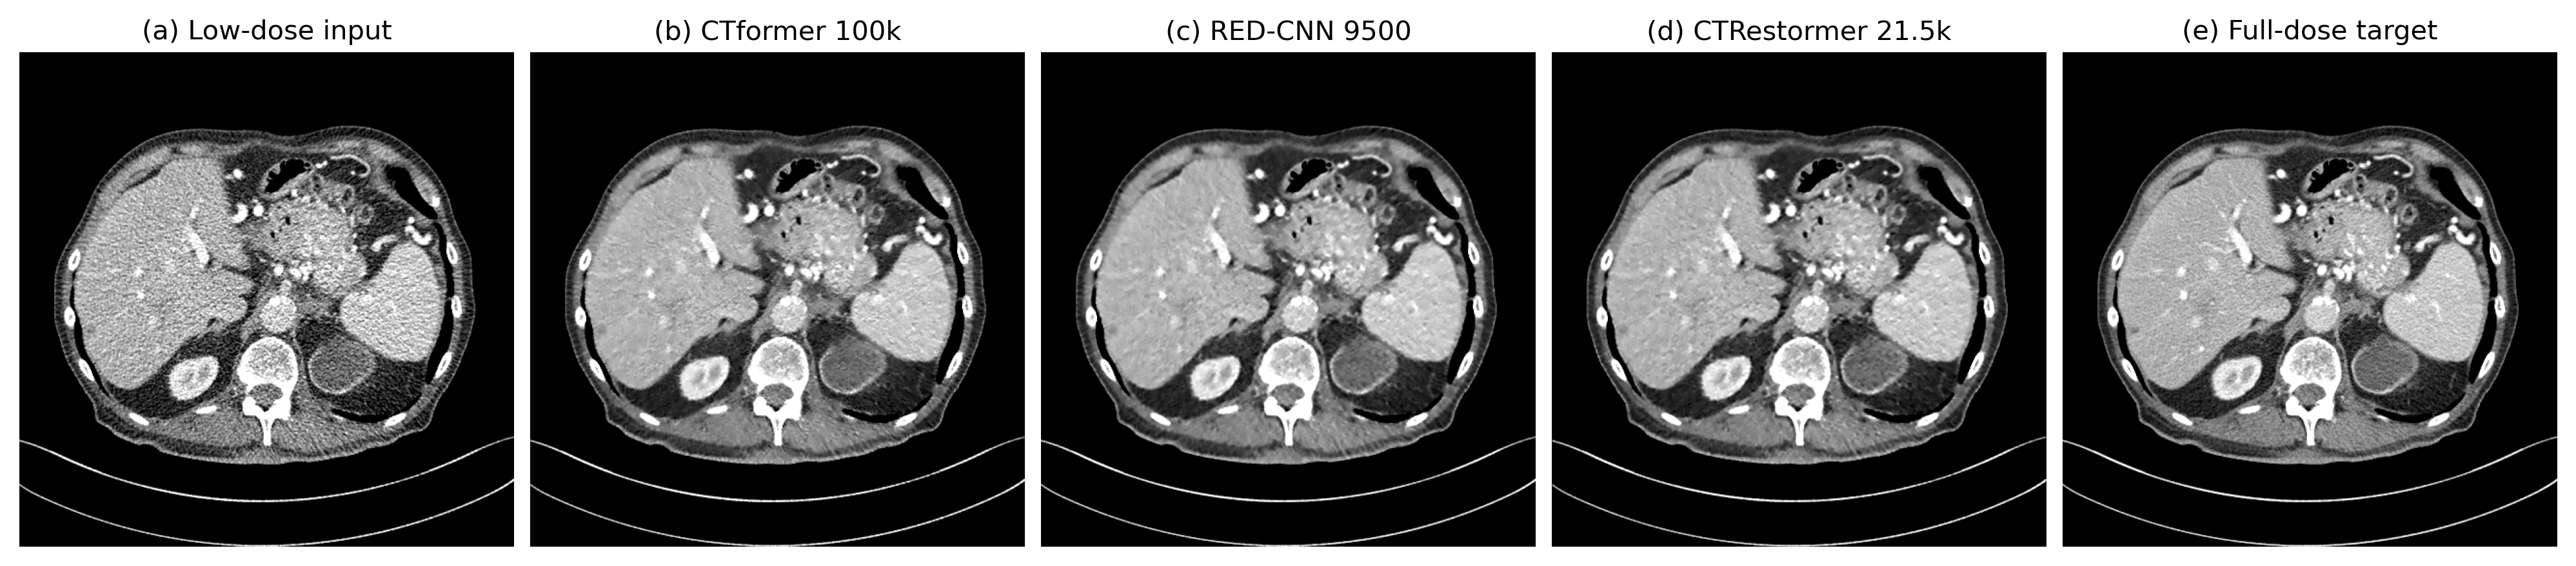
\includegraphics[width=0.95\textwidth]{images/qualitative_l506_180_comparison.png}
    \caption{Additional qualitative comparison for slice L506\_180. This slice has the highest low-dose to full-dose RMSE among the inspected L506 slices, so it is useful for comparing denoising behavior under stronger visible noise.}
    \label{fig:qualitative_l506_180}
\end{figure}

\section{Training Curve}

Figures \ref{fig:ctrestormer_loss_curve} show the logged training loss trends for CTRestormer. 

\begin{figure}[!htbp]
    \centering
    
\includegraphics[width=0.78\textwidth]{images/ctrestormer_loss_curve.png}
    \caption{Training loss trend from the CTRestormer run. The plotted loss is the logged loss.}
    \label{fig:ctrestormer_loss_curve}
\end{figure}
